\documentclass[11pt]{beamer}

\usepackage[english]{babel}
\usepackage[T1]{fontenc}
\usepackage[utf8]{inputenc}
\usepackage{mathtools}                       % matma
\usepackage{amsfonts,amsmath,amssymb,amsthm} % matma


\title{Bayesian games}
\author{Stanisław Bitner, Aleksander Wojsz}
\date{\today}

\usetheme{Warsaw}
\usecolortheme{orchid}

\setbeamertemplate{footline}[Warsaw]
\setbeamertemplate{headline}{}
\setbeamertemplate{page number in head/foot}[totalframenumber]
\setbeamertemplate{navigation symbols}{}


\begin{document}


\frame{\titlepage}



\begin{frame}
    \frametitle{Bayesian games - intuitive definition}

    \only<1>{
    So far we have assumed that each player knows the payoff of other players. 
    Ex. Prisoners dilemma. We didn't know whether our colleague will cooperate
    with police, but we knew payoffs for all possibilities.

    \vspace{5mm}

    Closer to real life are games with incomplete information (uncertainty about
    payoffs) called Bayesian Games.
    }

    \only<2>{
    In games with incomplete information we have
    \begin{itemize}
        \item Players
            \begin{itemize}
                \item One player can have multiple types each having different
                    payoffs
                \item Player has probability assigned for each type of his
                    opponent
                \item Player 2 knows that player 1 has beliefs. \\
                Player 1 knows that player 2 knows that player 1 has beliefs. \\
                Player 2 knows that player 1 knows that player 2 knows that player 1 has beliefs. \\
                ... and so on
            \end{itemize}
        \item Actions
        \item Payoffs
    \end{itemize}

    \vspace{5mm}

    So in short, the difference is these types and beliefs about these types.
    }
    \only<3>{
    Bayesian game eliminates infinite loops in situations where players try to
    predict each other's thoughts. For instance, a player might think, "If
    I expect $\textit{player B}$ to take a certain action, then $\textit{player
    B}$ will predict that I expect this action, so I need to predict
    $\textit{player B's}$ prediction", and so on. Bayesian games simplify this
    by assigning probability weights to each outcome.
    }
\end{frame}


\begin{frame}
    \frametitle{Example on Battle of the Sexes}

    \begin{figure}
        \centering
        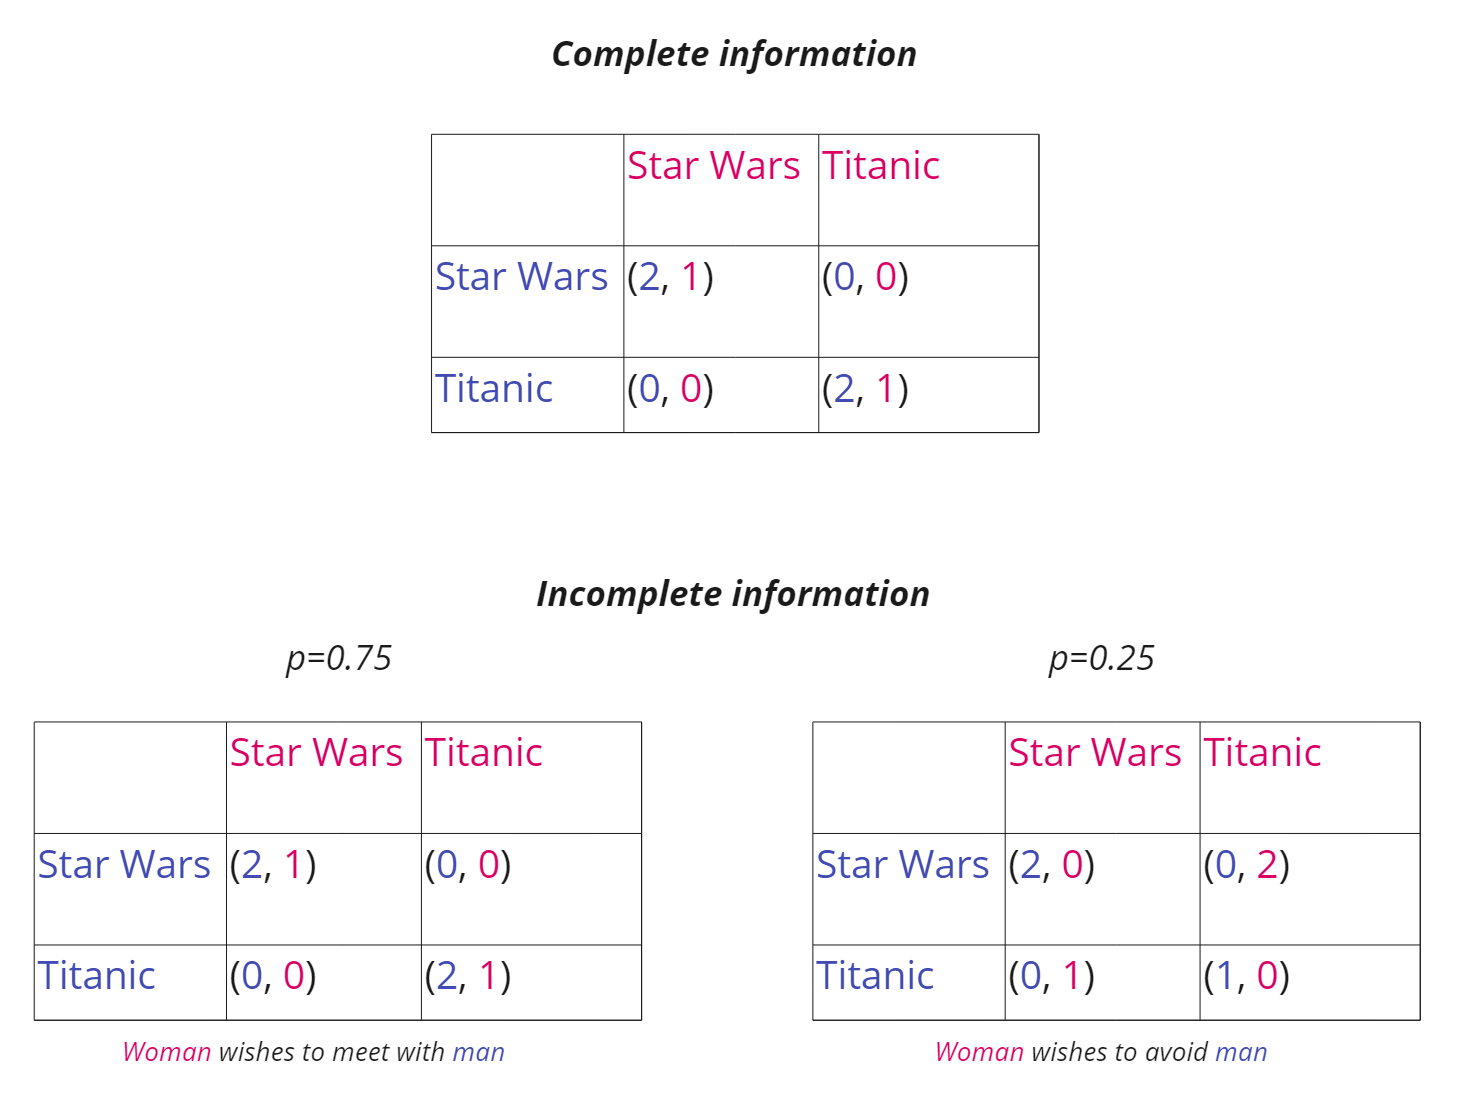
\includegraphics[width=0.8\textwidth]{assets/movies.png}
    \end{figure}
    
    \vspace{5mm}

\end{frame} 


\begin{frame}
    \frametitle{Tree representation}

    \begin{figure}
        \centering
        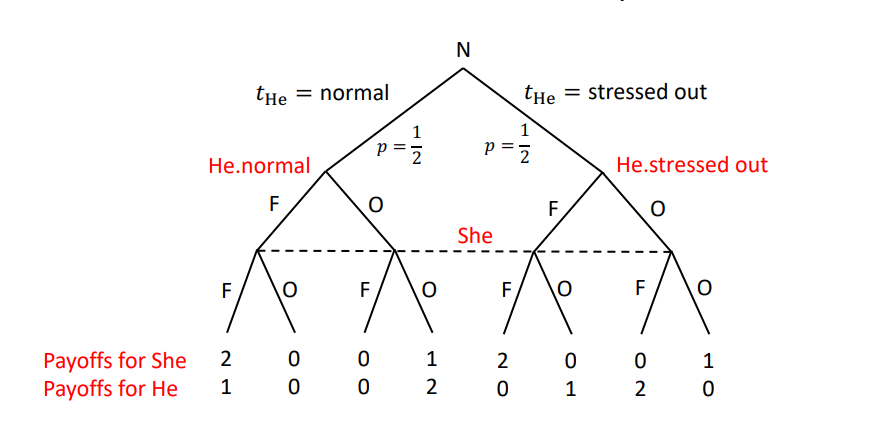
\includegraphics[width=1.0\textwidth]{assets/tree.png}
    \end{figure}
    
    \vspace{5mm}

    \textbf{Watch out! Here she prefers football and he prefers opera.}

\end{frame} 


\begin{frame}
    \frametitle{Example on Sheriff's dilemma}

    \only<1>{
    \vspace{10mm}
    
    \begin{figure}
        \centering
        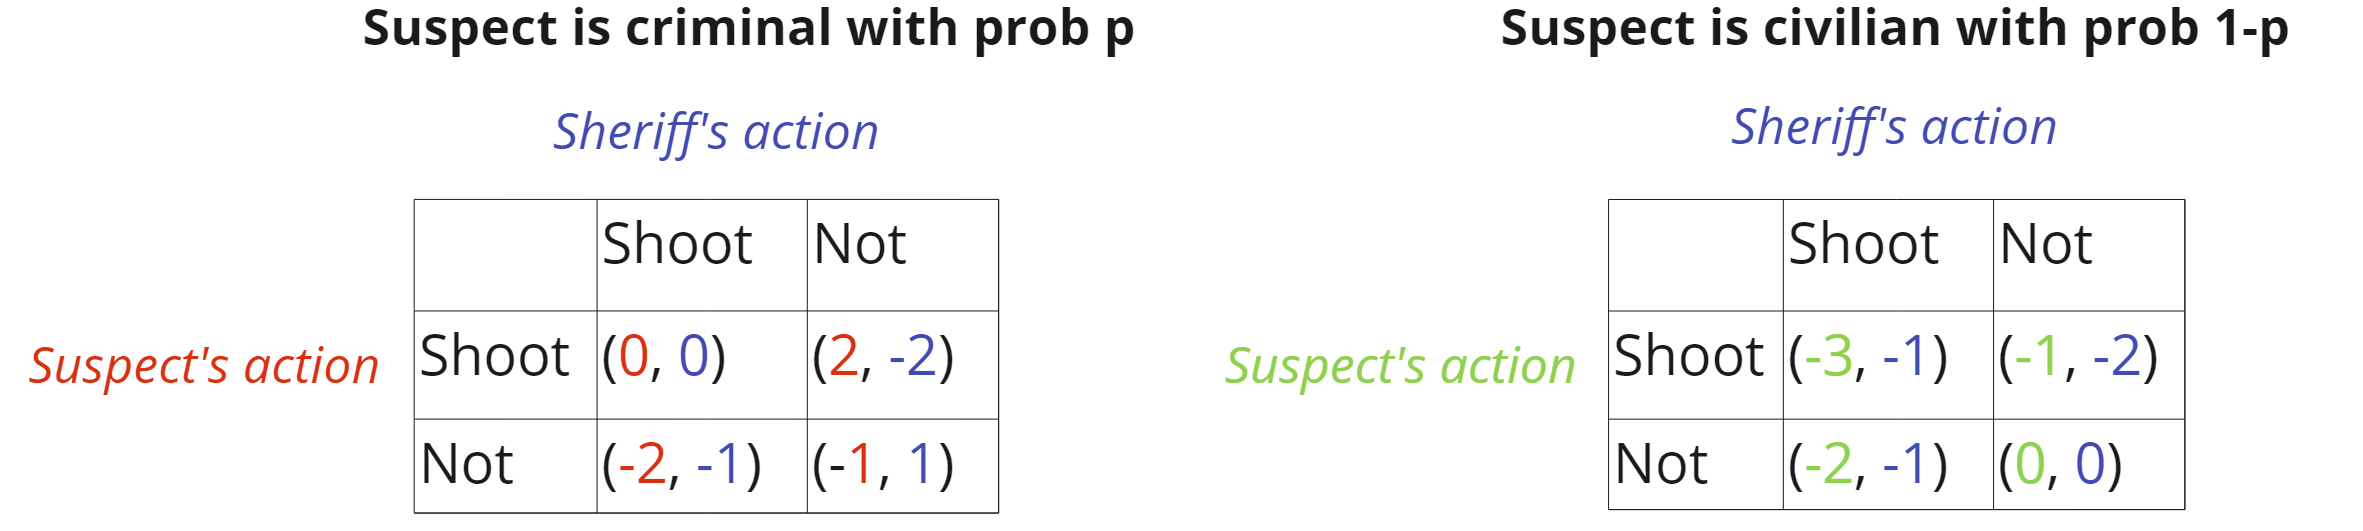
\includegraphics[width=1.0\textwidth]{assets/sheriff.png}
    \end{figure}

    \vspace{20mm}
    
    \begin{figure}
        \centering
        
\includegraphics[width=0.5\textwidth]{assets/gunfight.jpg}
    \end{figure}
    }
    
    \only<2>{
    \begin{figure}
        \centering
        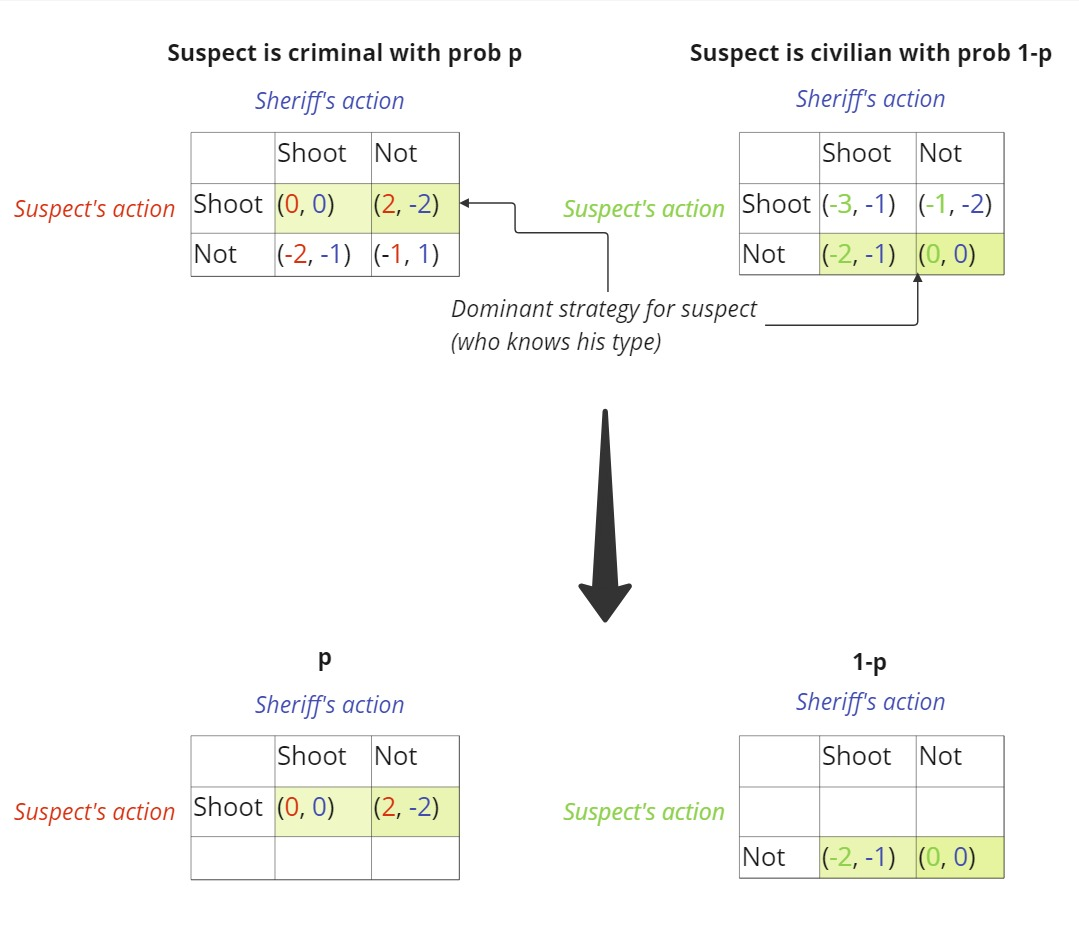
\includegraphics[width=0.8\textwidth]{assets/sheriff2.jpg}
    \end{figure}

    \vspace{5mm}
    }
    
    \only<3>{
    \begin{figure}
        \centering
        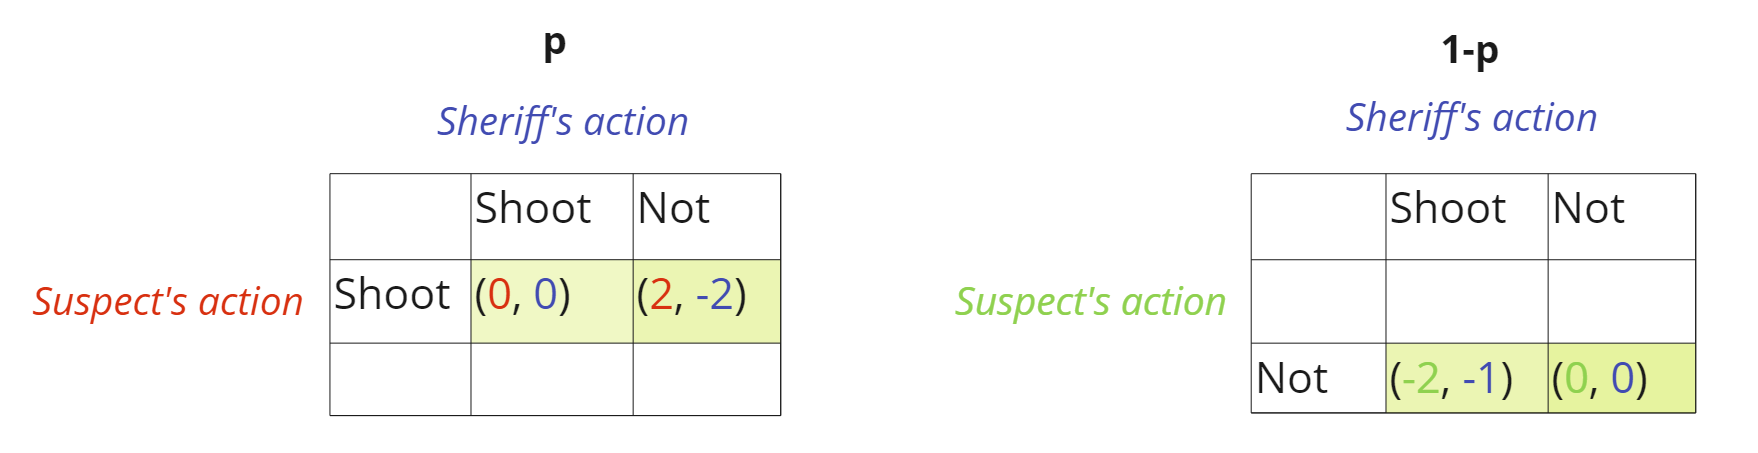
\includegraphics[width=1.0\textwidth]{assets/sheriff3.png}
    \end{figure}

    \vspace{5mm}

    Expected payoff for sheriff if he shoots:
    $$0 \cdot p + (-1)(1-p) = p - 1$$
    and if he does not shoot:
    $$-2 \cdot p + 0 \cdot (1-p) = -2p$$

    Therefore, sheriff should shoot only when 
    $$ p-1 > -2p \qquad\qquad p > \frac{1}{3} $$
    }
    
\end{frame} 



\begin{frame}
    \frametitle{Mathematical definition}

    A Bayesian game is defined by $(N,A,T,p,u)$, where:
    
    \vspace{5mm}
    \begin{itemize}
        \item \textbf{$N$ - Set of players}
        \vspace{2mm}
        \item \textbf{$a_i \in A$ - Actions:} The set of actions available to Player $i$.
        \vspace{2mm}
        \item \textbf{$t_i \in T$ - Types:} The set of types for player $i$. Captures the private information a player can have.
        \vspace{2mm}
        \item \textbf{$u$ - Payoff functions:} Assign a payoff to a player given their type and the action profile.
        \vspace{2mm}
        \item \textbf{$p$ - Types probabilities:} Where $p(t) = p(t_1, \ldots, t_N)$ is the probability that Player 1 has type $t_1$ and Player $N$ has type $t_N$.
    \end{itemize}

\end{frame}

\begin{frame}
    \frametitle{{Mathematical definition example}}
    \begin{itemize}
        \item $N = \{\text{Suspect, Sheriff}\}$
        \item $A_{\text{Suspect}} = \{\text{Shoot, Not}\}$, $A_{\text{Sheriff}} = \{\text{Shoot, Not}\}$
        \item $T_{\text{Suspect}} = \{\text{Criminal, Civilian}\}$, $T_{\text{Sheriff}} = \{ \text{Default} \}$
        \item $p_{\text{Criminal}} = p$, $p_{\text{Civilian}} = (1 - p)$
        \item Payoffs $u$ are the tables we have seen before
    \end{itemize}
\end{frame}


\begin{frame}
    \frametitle{Extensions}
    \begin{itemize}
        \item She and He have an arbitrary number of types each.
        \item There are more than two players.
        \item Players choose sequentially. The player playing second can observe the action, but
        not the type of the player playing first.

    \end{itemize}
\end{frame}


\begin{frame}
    \frametitle{Impact of Asymmetric Information on the Market}

    \only<1>{
    \begin{itemize}
        \item There are two cars:
        \begin{itemize}
            \item A high-quality car worth \$100,000, sold for \$100,000.
            \item A defective car with hidden flaws worth \$50,000, also sold for \$100,000.
        \end{itemize}
        \item The buyer does not know which car has hidden flaws, so they take this into account and negotiate a price in the middle: \$75,000.
        \item Since sellers of high-quality cars cannot sell them for lower prices than the cars are worth, they leave the market. Only low-quality cars can be sold for lower prices.
        \item As a result, the average quality and price in the market decrease.
        \item This cycle repeats until buyers only want cars for free.
    \end{itemize}
    }
    
    \only<2>{
    \begin{figure}
        \centering
        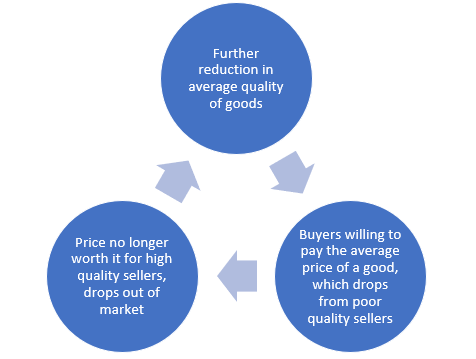
\includegraphics[width=0.6\textwidth]{assets/cycle_of_market.png}
    \end{figure}

    In Poland, nearly twice as many used cars are sold as new ones, so there
    are, of course, ways to deal with this problem, such as warranties.
    }
\end{frame}

\begin{frame}{Resources}
    \begin{itemize}
        \item \url{https://en.wikipedia.org/wiki/Bayesian_game}
        \item \url{https://www.ehu.eus/iaguirre/Chapter\%201.\%20Bayesian\%20Games\%20in\%20Normal\%20Form.pdf}
    \end{itemize}
\end{frame}

\end{document}
